\chapter{Herní API}
Tato část softwaru je programována za účelem jednoduché tvorby komplexních outdoorových her.
Toho se snaží dosáhnout velkou modulárností a~zaměřením na principy OOP.

\section{Stránky}

Pro vytváření jednoduchých her a~uživatelsky přívětivých menu je implementován systém stránek (Page) a~aplikací (App).

\subsection{Page}

Stránka je soubor barev jednotlivých pozic na displeji (LED kruh) společně s~akcemi při jejich zvolení, nebo při jiné události.\footnote{Zatřesení BlackBoxem, povel z případné nadřazené jednotky \dots}
Prováděné akce jsou uživatelem definované funkce.
Pro pohodlnost je však implementováno několik základních akcí, například blikání.

Speciálním typem předdefinované akce je Link.
Link je způsob propojování více stránek mezi sebou, kupříkladu pokud zvolíte specifickou pozici na první stránce, přehodí vás Link na stránku druhou.\footnote{Toto se dá použít pro tvorbu jednoduchých bludišť.}
Přehození kontextu na jinou stránku je vždy poslední provedená akce vyvolaná událostí.

\subsection{App}

Aplikace je jednoúčelový podprogram zapadající do systému stránek, chová se vlastně jako speciální Page.
Zatímco page je statická (v průběhu kódu se zásadně nemění), aplikace je velmi dynamická.
Do aplikace se dá jednoduše naprogramovat, cokoliv bude uživatel vyžadovat, kupříkladu:
\begin{itemize}
    \item Navigace
    \item Logické hádanky
    \item Hodiny
    \item A~mnoho dalších \dots
\end{itemize}

\section{Zamykání}

Ačkoliv může slovo zamykání na elektronické sejfu, kterým BlackBox je, vyvolat myšlenku o~zamykání tohoto sejfu, není tomu tak.
Funkce zamykání funguje se spoustou věcí.
Primárně však tento systém funguje inhibitor událostí a~přepínání mezi instancemi Page a~Application.

\subsection{Latch}
Latch je zamykací primitivum.
Každý typ Latch má jinou odemykacím/zamykací podmínku.
Mohou být vázané na některý z~senzorů prostředí, Orientation latch lze nastavit, aby k odemknutí vyžadoval otočení BlackBoxu čelem k severu, což zjistí díky zabudovanému magnetometru.

Dalším příkladem může být Time Interval Latch, která se odemkne v~případě, že aktuální čas je v~definovaném rozsahu.

Kromě senzorů však může být Latch ovládán také z~jiných částí kódu, nebo dokonce z~úplně jiného zařízení, k~tomu slouží Remote Latch.

\subsection{Lock}

Lock je třída, která spravuje jednotlivé Latch objekty a~v závislosti na svém typu se odemyká a~zamyká v~závislosti na stavu podřazených Latch.
Mezi tyto typy patří například:
\begin{itemize}
    \item All -- AND
    \item None -- NAND
    \item AtLeast(n) -- alespoň n Latch musí být odemknuto
    \item Weighted(x) -- Každé latch je přiřazena váha, součet vah odemčených Latch potom musí být >= x
    \item A~další \dots
\end{itemize}
Lock také může být vložen do dalšího Lock objektu.

\begin{figure}[H]
    \begin{small}
        \begin{center}
            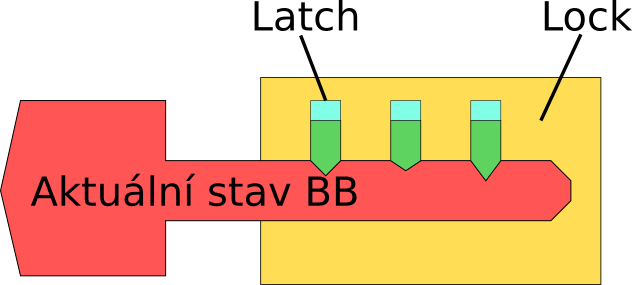
\includegraphics[width=0.95\textwidth]{img/lock.png}
        \end{center}
        \caption{Idea zámku}
        \label{fig:lock}
    \end{small}
\end{figure}

\newpage

\section{Příklady použití}

\lstinputlisting[language=C++, caption=Ukázka propojování stránek]{code/pageSimple.cpp}

\begin{figure}[H]
    \begin{small}
        \begin{center}
            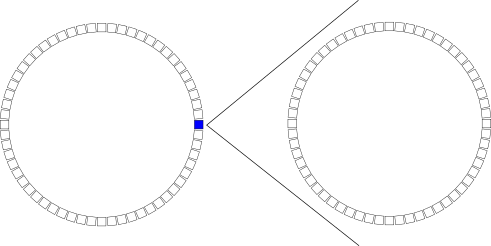
\includegraphics[width=0.95\textwidth]{img/pageLink.png}
        \end{center}
        \caption{Vizualizace výsledku ukázky propojování stránek}
        \label{fig:pageLink}
    \end{small}
\end{figure}

\newpage

\lstinputlisting[language=C++, caption=Ukázka propojování aplikací]{code/appSimple.cpp}

\begin{figure}[H]
    \begin{small}
        \begin{center}
            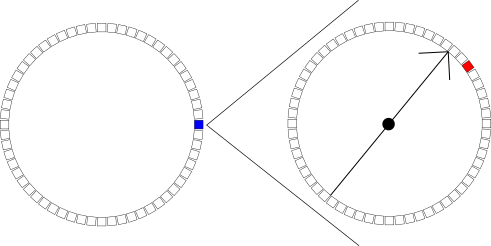
\includegraphics[width=0.95\textwidth]{img/appLink.png}
        \end{center}
        \caption{Vizualizace výsledku ukázky propojování aplikací}
        \label{fig:appLink}
    \end{small}
\end{figure}

\newpage

\lstinputlisting[language=C++, caption=Ukázka práce s herním API]{code/page.cpp}

\newpage

Pro potřeby této práce je \textbf{synchronní hra} taková hra k~jejímuž hraní je potřeba interakce hráčů v~reálném čase ať už s~"prostředím", nebo mezi sebou.
\textbf{Asynchronní} je poté hra, která nevyžaduje interakce v~reálném čase.

\subsection{Synchronní hry}

\subsubsection{Lights out/Večerka}

Hraje se v~noci s~BlackBoxy rozmístěnými v~mřížce na louce, část BlackBoxů svítí a~část ne.
Při zmáčknutí BlackBoxu se změní stav daného BlackBoxu spolu se stavy okolních BlackBoxů podle předem daného pravidla.
Cílem je vypnout všechny světla.

\subsubsection{Path of light/Světelná cesta}

Pro efekt je lepší hrát tuto hru v~noci.
Každý hráč má svůj BlackBox.
V~prostoru jsou rozmístěny záda pro BlackBox v~předem daných polohách.
V~závislosti na věku hráčů, herním čase a~dostupné prostoru může být herní plocha rozlehlá i~několik set metrů.
Je několik počátečních pozic.

Každý hráč má vygenerované bludiště, kde cesty jsou definované jako spojnice mezi BlackBoxy (toto bludiště se může autonomně měnit v~průběhu hry).
Když hráč dojde na stanoviště a~zasune svůj BlackBox do zad na stanovišti, zobrazí se mu možné směry, kterými se může vydat.
Hráč si jeden z~nich vybere a~BlackBox mu začne ukazovat přímou spojnici ke stanovišti v~daném směru.
Pokud hráč sejde z~originální přímé spojnice, může si opravit směr na jakémkoliv dalším stanovišti.

Hráč vyhrává, pokud se dostane do středu bludiště.


\subsection{Asynchronní hry}

Typickým příkladem asynchronní hry jsou šifrovací hry, kdy hráči dostanou na vyluštění delší časový úsek, hra potom může být rozdělena na etapy.
Začátek etapy bude sloužit jako synchronizační a~vylučovací bod.
Tento způsob šifrovací hry snižuje potřebu koordinace, protože ji každý může řešit "až bude mít čas."
